%https://tex.stackexchange.com/questions/208819/embedding-images-in-tex-file-as-base64-strings

%Questo è il preambolo, dove si inseriscono i pacchetti e le impostazioni che servono per compilare il documento. Quanto scritto dopo il simbolo '%' è solo un commento e serve a fini dimostrativi.
\documentclass{article}
%\documentclass[a4paper, 13pt, oneside]{report}
\linespread{1.5} %interlinea
\pagestyle{plain}
\usepackage{chngpage}
\usepackage{booktabs}

\usepackage{geometry} %margini
\geometry{a4paper, top=3cm, bottom=3cm, left=3cm, right=3cm, bindingoffset=5mm}
\usepackage{graphicx}
\usepackage{siunitx}
\usepackage{subcaption}
\graphicspath{img/}
\usepackage{multicol} %più colonne
\usepackage{ragged2e} %allineamento testo

% italian is gay
%\usepackage[italian]{babel} %lingua principale

\usepackage{minitoc} %mini sommario a inizio capitolo
\nomtcrule





\usepackage{comment}








\usepackage{xpatch}
\usepackage{blindtext}


\makeatletter

\makeatother

\usepackage{fancyhdr}
\usepackage[export]{adjustbox}



\usepackage{hyperref} %hyperlink
\hypersetup{
    colorlinks=true,
    citecolor=cyan,
    linkcolor=black,
    urlcolor=black,
    pdftitle=Report - \VAR{info.name},
    pdfauthor=ghoozie,
    }

\usepackage{booktabs} %per le tabelle
\usepackage{multirow}
\usepackage[table,xcdraw]{xcolor}
\usepackage{graphicx}

\usepackage{lscape}
\usepackage{float}
\usepackage{wrapfig}

\begin{document}
\begin{titlepage}   % TITLEPAGE

\begin{center}
	{\scshape\Large\bfseries \, \par}
	\vspace{5cm}


	
\includegraphics{/app/img/Provins.png}\par



	\vspace{0,5cm}
	{\scshape\Large\bfseries Recommended Asset Allocation

	{\VAR{info.name}} | {\VAR{info.date}} \par}
	\vspace{0,5cm}
	{\scshape\normalsize Frontier Curve Optimal Portfolio Analysis

	Monte Carlo Simulation Of Returns

	Correlation Matrix \par}
\end{center}

	\begin{center}
\line(1,0){250}
\end{center}

	\begin{center}
	 	{
		\small{
		Prepared by Thomas K. Provins

		THOMAS.PROVINS@LPL.COM}
		\par}


	\vfill
\end{center}

	\vfill

% Bottom of the page
	{\begin{center}

	     1910 Cochran Road

	     Manor Oak 2 Suite 450

	     412.440.6949

	\end{center}}

\end{titlepage}


\tableofcontents    % PAGE1

\begin{center}
\vfill
\vfill

\end{center}
\justify

\newpage    % PAGE2

\section{Statistical Terminology \& Asset Class Descriptions}

\textbf{Expected Return} - Of an investing strategy is the amount of money you are expected to get back from your investment. For example, if 90 dollars is invested for 1 year with an expected return of 100 dollars, then in the average case the investment will yield back 100 dollars.


\vspace{.5cm}

\noindent \textbf{Risk} - Or standard deviation of an investing strategy is a measure of how much the return of an investment strategy will vary from it's expected return. For example, an investment strategy with an expected return of 20\% and a risk of 8\% will yield 112\% to 128\% return with a probability of 68.2\% , and 104\% to 136\% return with a probability of 94.4\%

\vspace{1cm}
\large
\noindent \textbf{The 18 Asset Classes : }
\normalsize
\vspace{.5cm}
\begin{adjustwidth}{0in}{0in}  % adjust the L and R margins
\begin{tabular}{lll}   %\toprule
    \textbf{Asset Class} & \textbf{Index} & \textbf{Description}\\ \midrule

    \BLOCK{ for key, value in book.iterrows() }
        \VAR{value.assetclass} & \VAR{value.latex} & \VAR{value.description} \\\midrule
    \BLOCK{ endfor }


\end{tabular}
\end{adjustwidth}


\newpage  % PAGE3

\section{Investment Profile}

\vspace{.5cm}

\large
\begin{tabular}[t]{l}
\vspace{.1cm}\\


\noindent\textbf{General Information}\\
\noindent Name : {\VAR{info.name}} \\
\noindent Birthday : {\VAR{info.birthday}} \\
%\noindent Purpose : Retirement \\
\noindent Time Frame : {\VAR{info.term}} \\
\noindent Available Funds : {\VAR{info.wealth}} \\
\noindent Preferred Risk : $\pm$ {\VAR{redrisk}} Yearly \\
\end{tabular}
\normalsize

\hspace*{-0.5cm}
\begin{tabular}{lll}

\vspace{1cm}\\
\large \textbf{Recommended Asset Classes:} & & \normalsize \vspace{0.3cm}\\

     \textbf{Asset Class} & \textbf{Index} & \textbf{Description}\\ \midrule

    \BLOCK{ for key, value in redbook.iterrows() }
         \VAR{value.assetclass} & \VAR{value.latex} & \VAR{value.description} \\\midrule
    \BLOCK{ endfor }

\end{tabular}


\vspace{1cm}


\newpage

\section{Prescribed Allocation Changes}
\begin{center}

  \begin{tabular}{ccc}
  \hspace*{-1.5cm}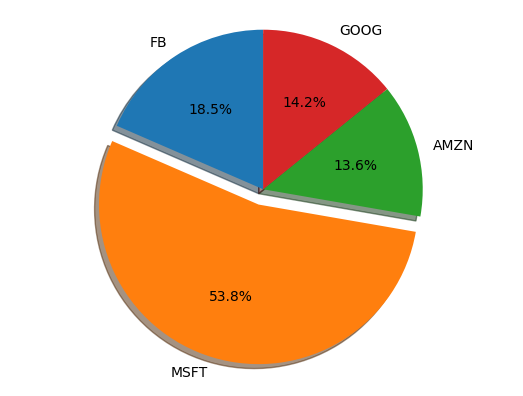
\includegraphics[width=.55\linewidth]{/app/plts/pie.png}
    & \hspace{0.5cm}&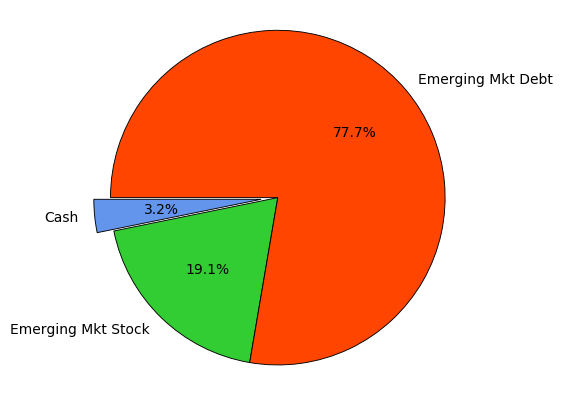
\includegraphics[width=.55\linewidth]{/app/plts/piefuture.png} \\
    (a) Current Portfolio && (b) New Portfolio
  \end{tabular}


\vspace{0.3cm}




\normalsize

\hspace*{-1.5cm}
\begin{tabular}{lccc}
    \textbf{Asset Class} & \textbf{Current} & \textbf{Suggested} & \textbf{Change}\\ \midrule


    \BLOCK{ for key, value in ybook.iterrows() }
        \VAR{value.assetclass} & \VAR{value.allocation} & \VAR{value.recommended} & \VAR{value.change.rjust(100)} \\ \midrule
    \BLOCK{ endfor }


\end{tabular}
\end{center}

%1. Large Cap Growth Stocks - Over invested by \$34,323.34. \\
%\,\,\,\,\,\, Reduce your holdings (\$56,372.43$).\\



\newpage    % PAGE4

\section{Performance Improvements Of Prescribed Portfolio}

Below are 7 year simulation results of your current investing strategy versus the investment strategy prescribed in this report. \\
Change In Expected Return : {\VAR{retchange}}\\
Change in Risk : {\VAR{riskchange}}

\vspace{.4cm}
\begin{center}


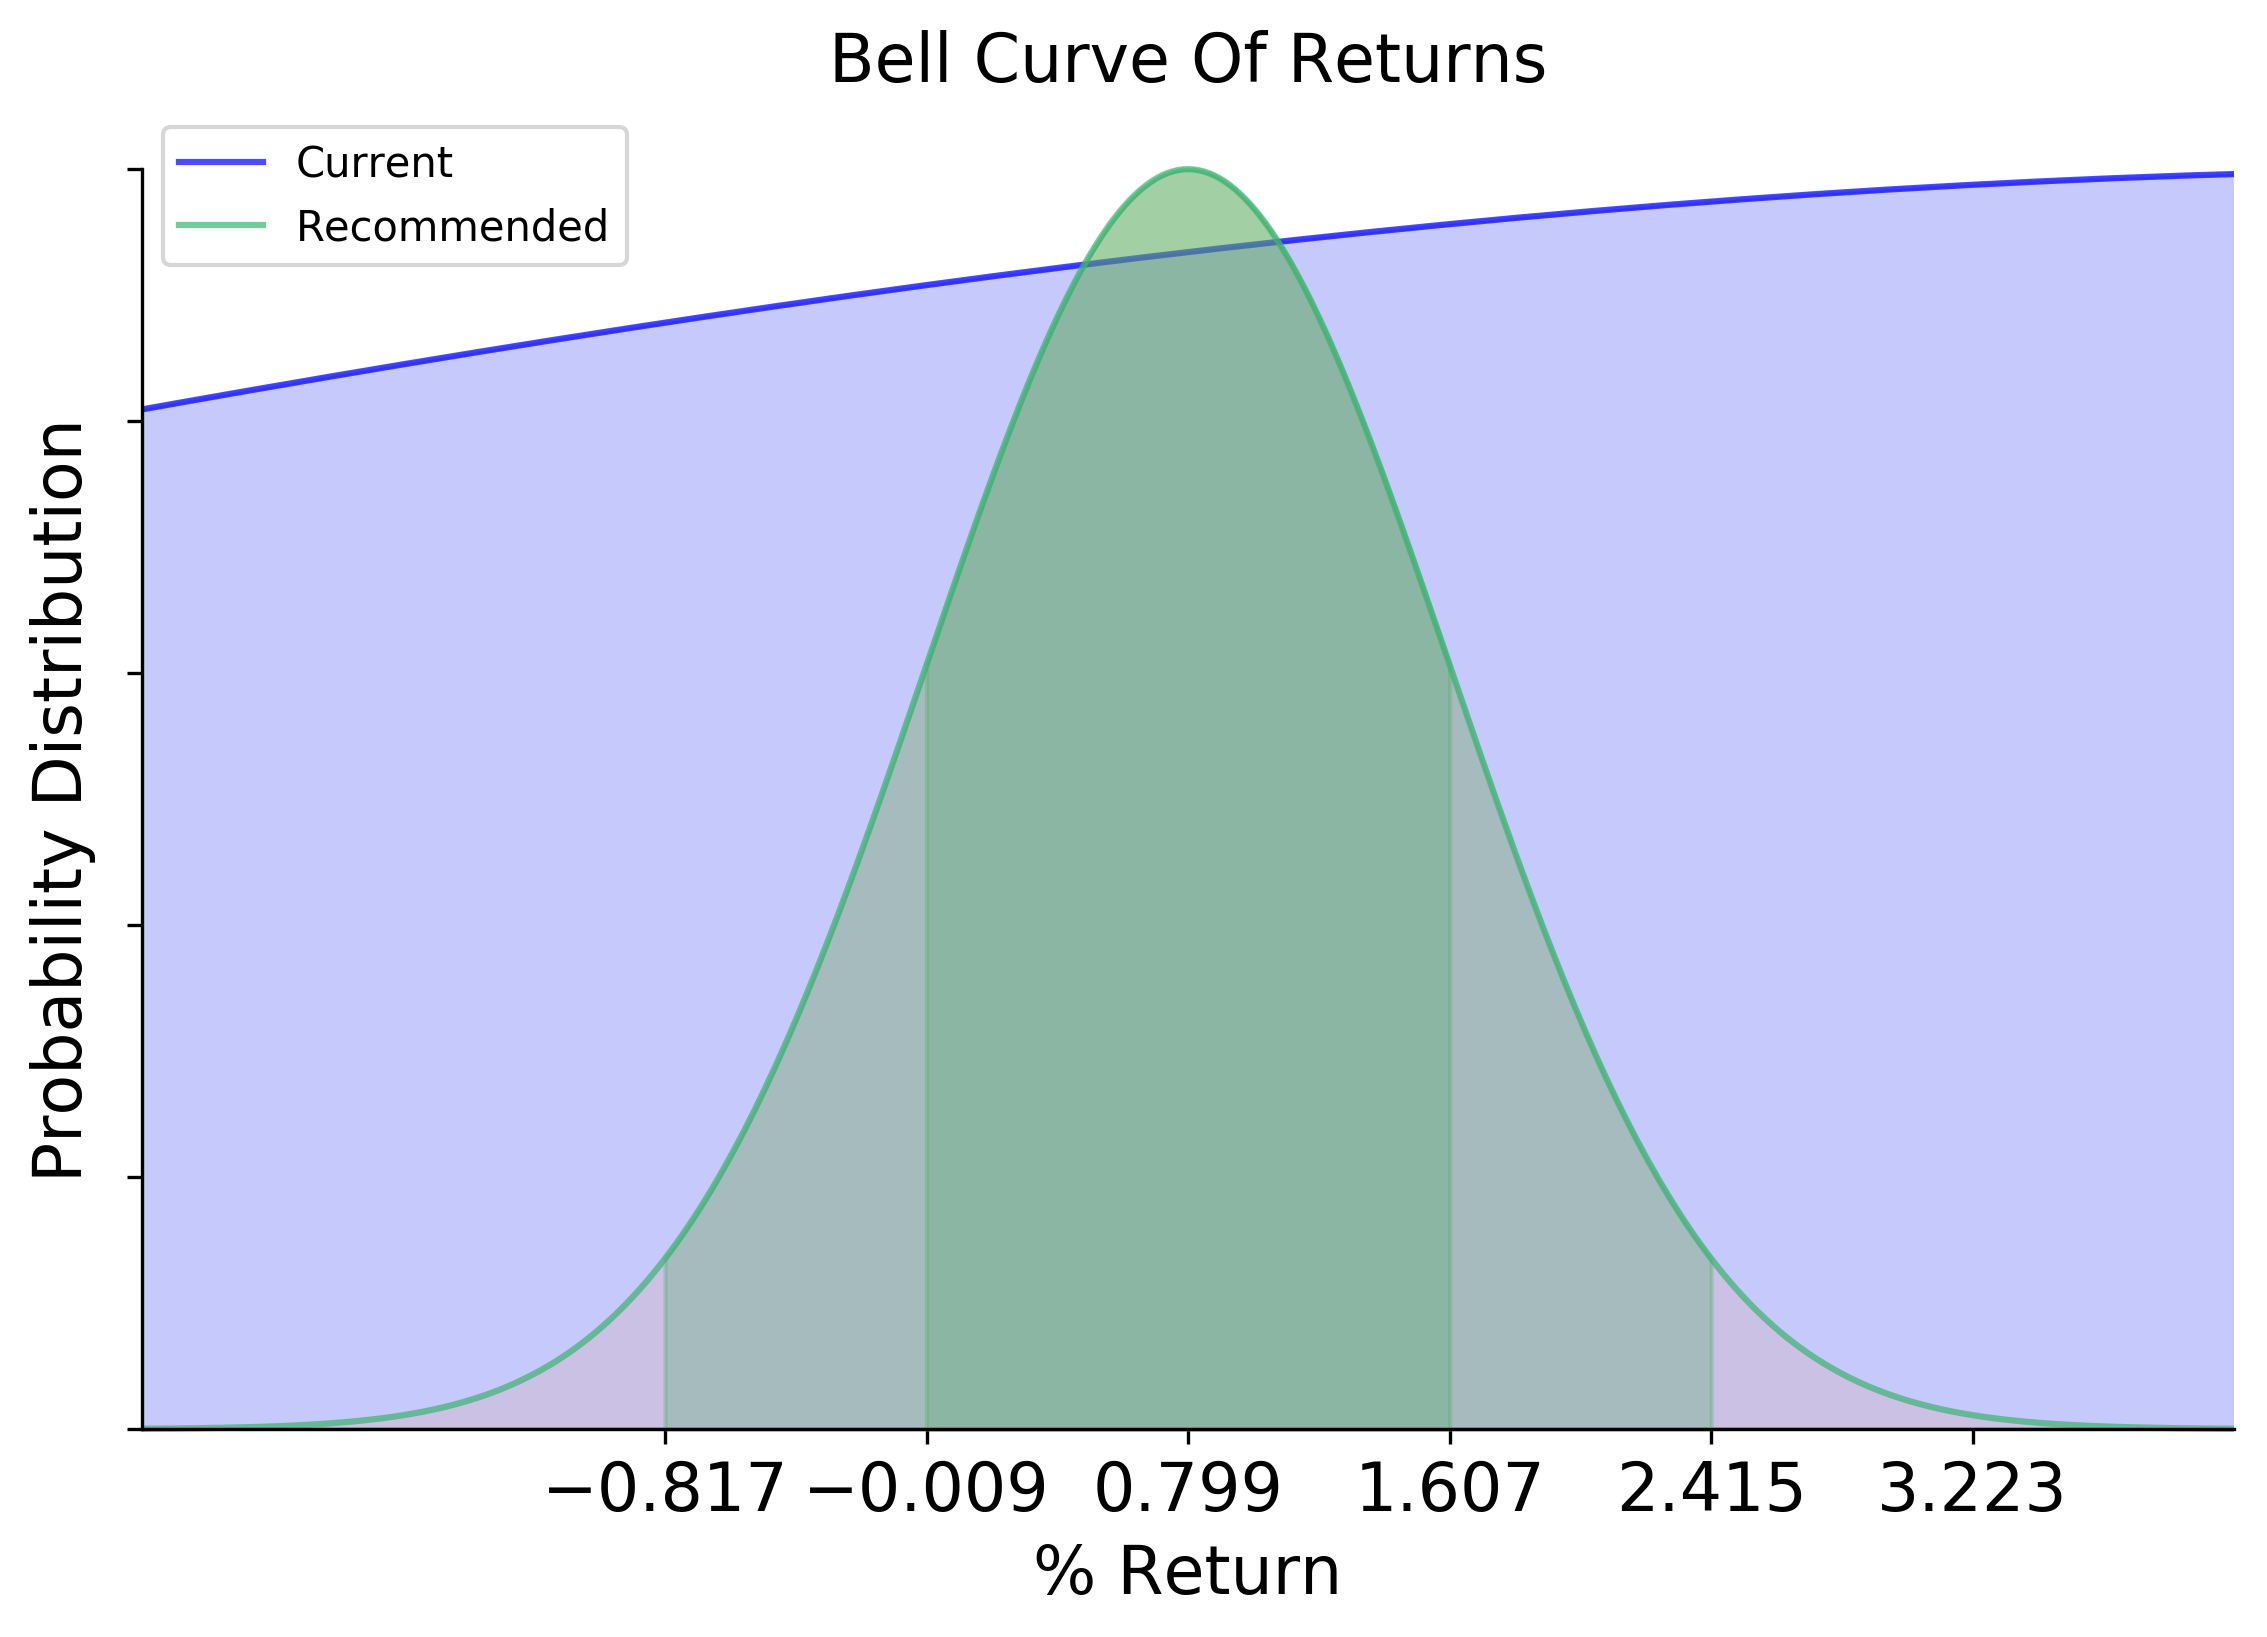
\includegraphics[width=.8\linewidth]{/app/plts/bellcompare.png}\par

\vspace{.5cm}

\hspace*{-1cm}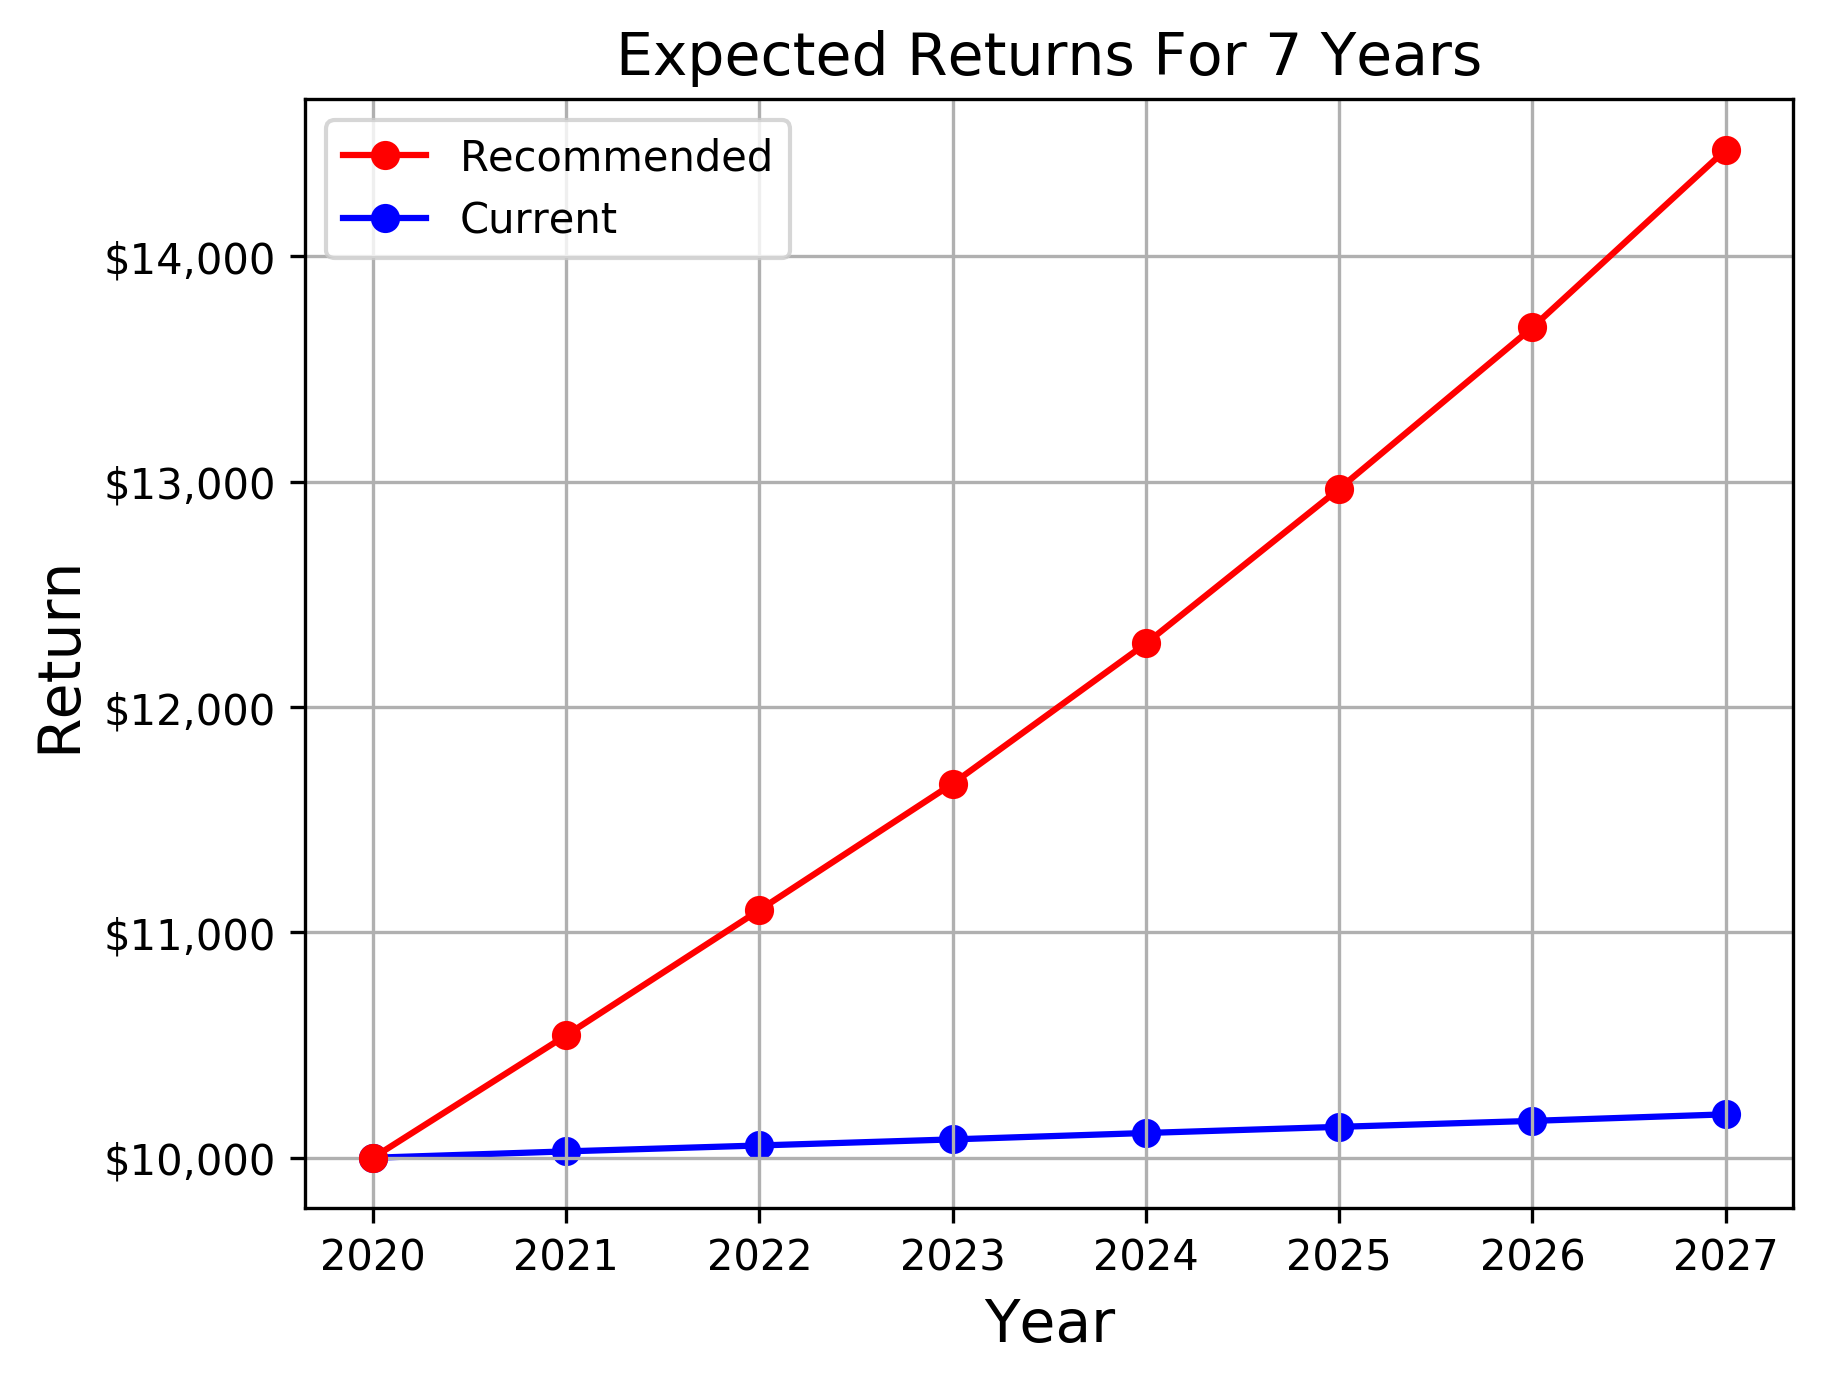
\includegraphics[width=.8\linewidth]{/app/plts/line7.png}\par
\end{center}

\newpage    %PAGE5

\section{Current Portfolio Overview - Statistical Analysis}

\vspace{1.5cm}

%https://tex.stackexchange.com/questions/257337/how-to-have-a-figure-with-multiple-groups-of-image-and-each-image-with-individua

\begin{adjustwidth}{-.3in}{0in}% adjust the L and R margins by 1 inch
\vspace*{-1cm}

\begin{center}
  \begin{tabular}{c}
    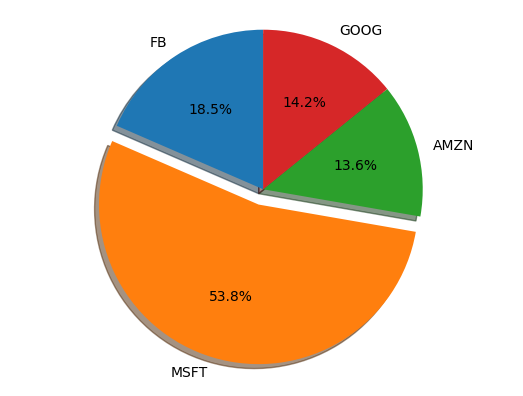
\includegraphics[width=.5\linewidth]{/app/plts/pie.png}
  \end{tabular}
  \end{center}

  \begin{center}
        Portfolio Breakdown
      %(b) Projected Returns (Monte Carlo)
  \end{center}

\vspace{.7cm}


\begin{center}
  \begin{tabular}{lcr}
  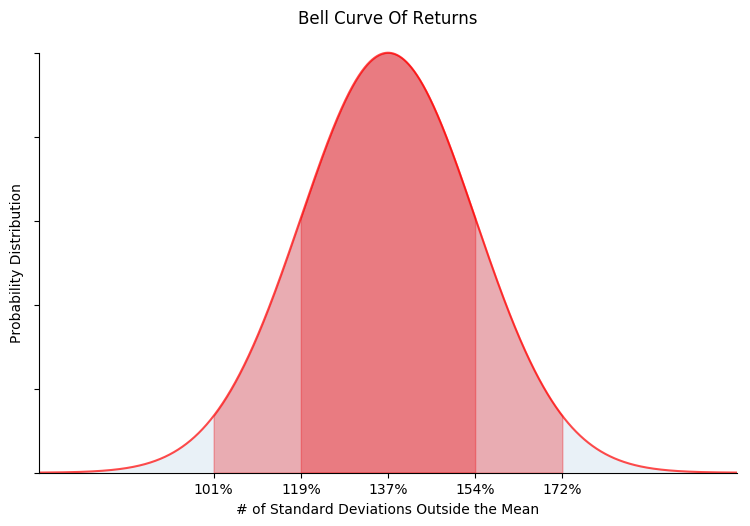
\includegraphics[width=.45\linewidth]{/app/plts/bell.png}
    & \hspace{1cm }&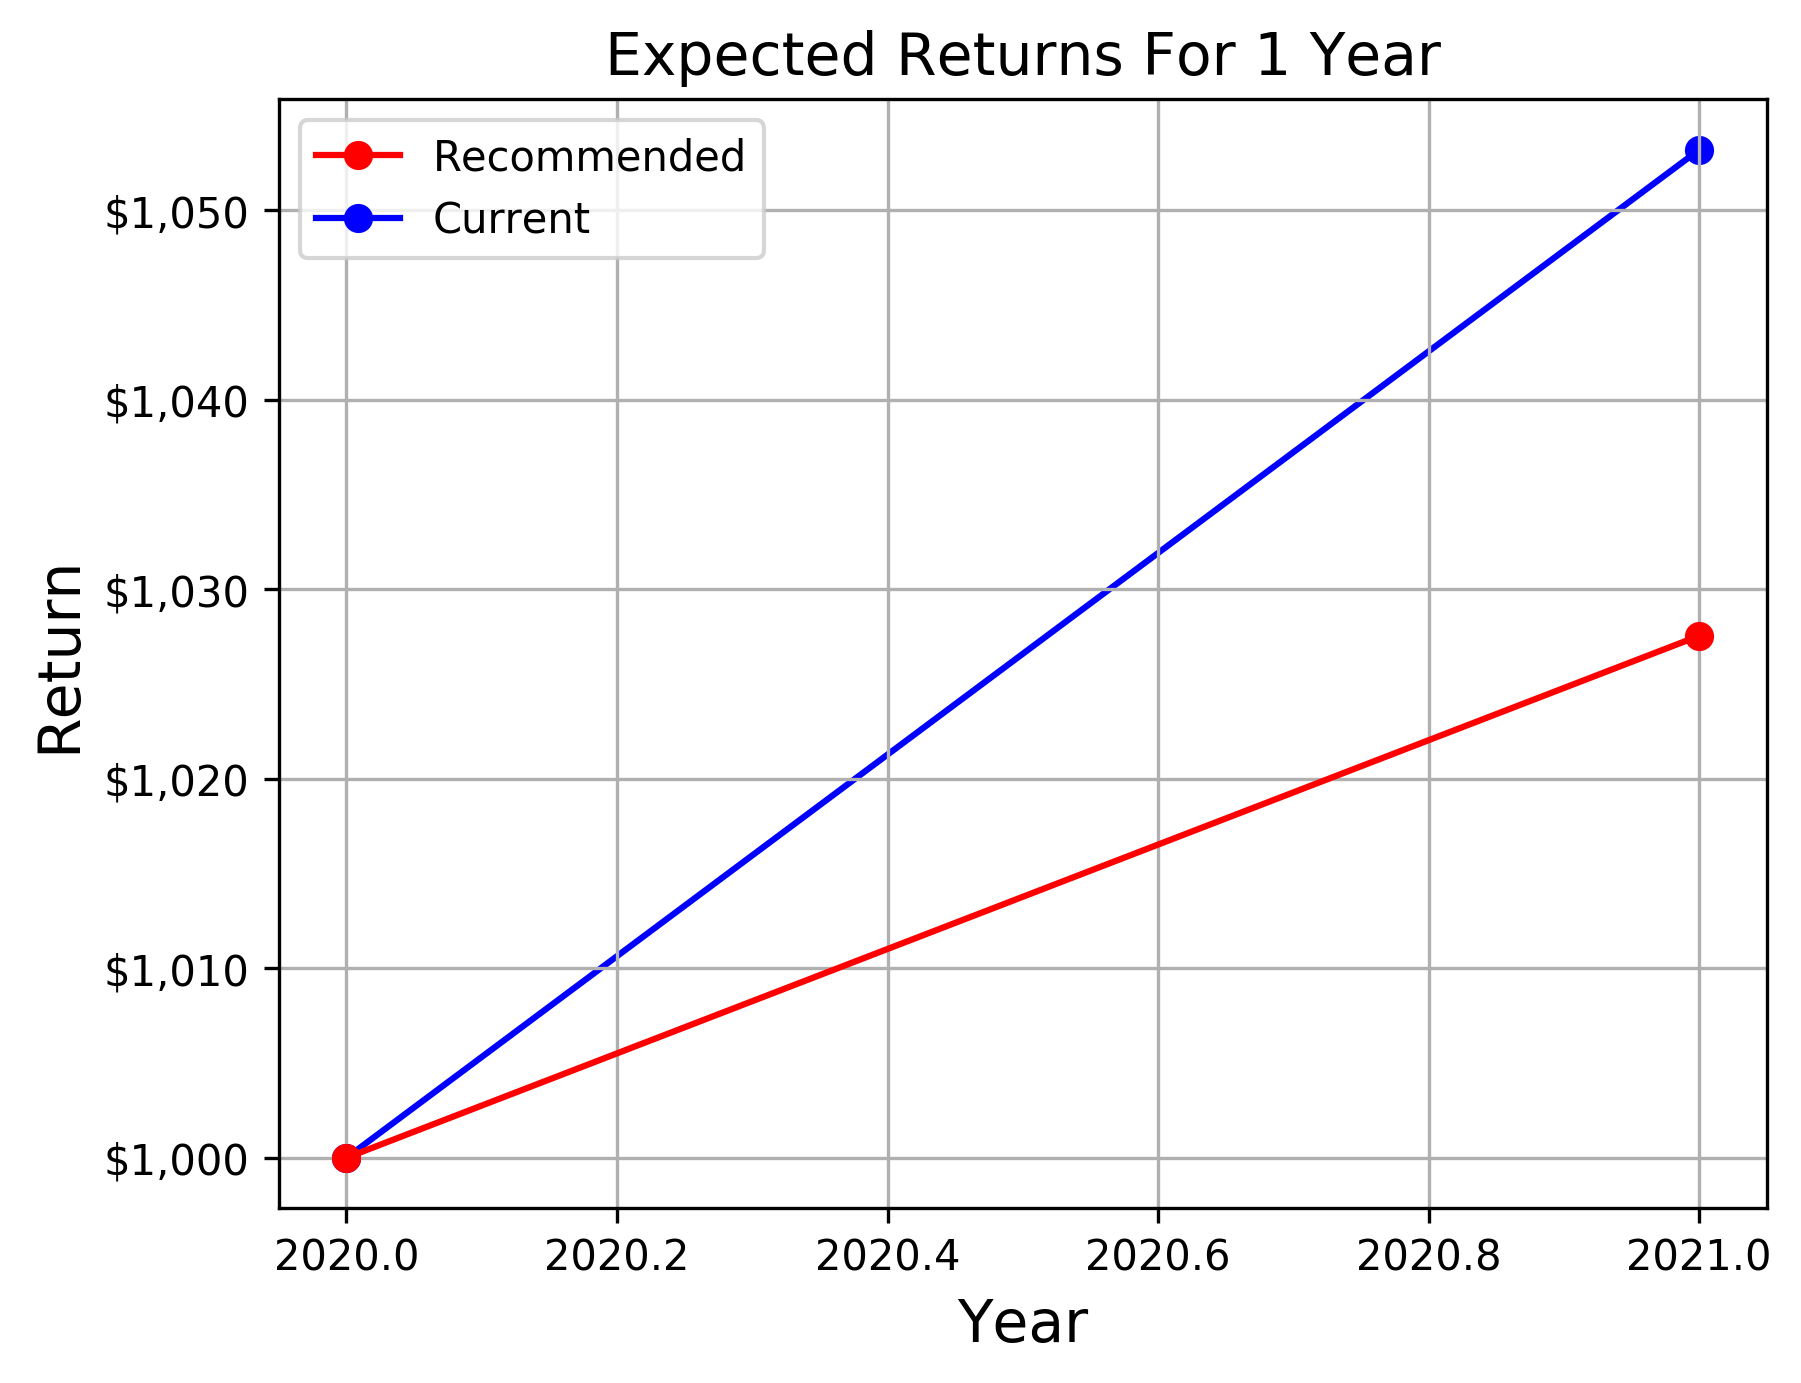
\includegraphics[width=.45\linewidth]{/app/plts/line1.png}
  \end{tabular}
  \end{center}

  \begin{center}
      (a) Current Portfolio 1 Year Projections
      %(a) Returns of Current Portfolio
      %(a) Bell Curves Of Expected Return
  \end{center}

  \vspace{.7cm}


\begin{center}
  \begin{tabular}{lcr}
  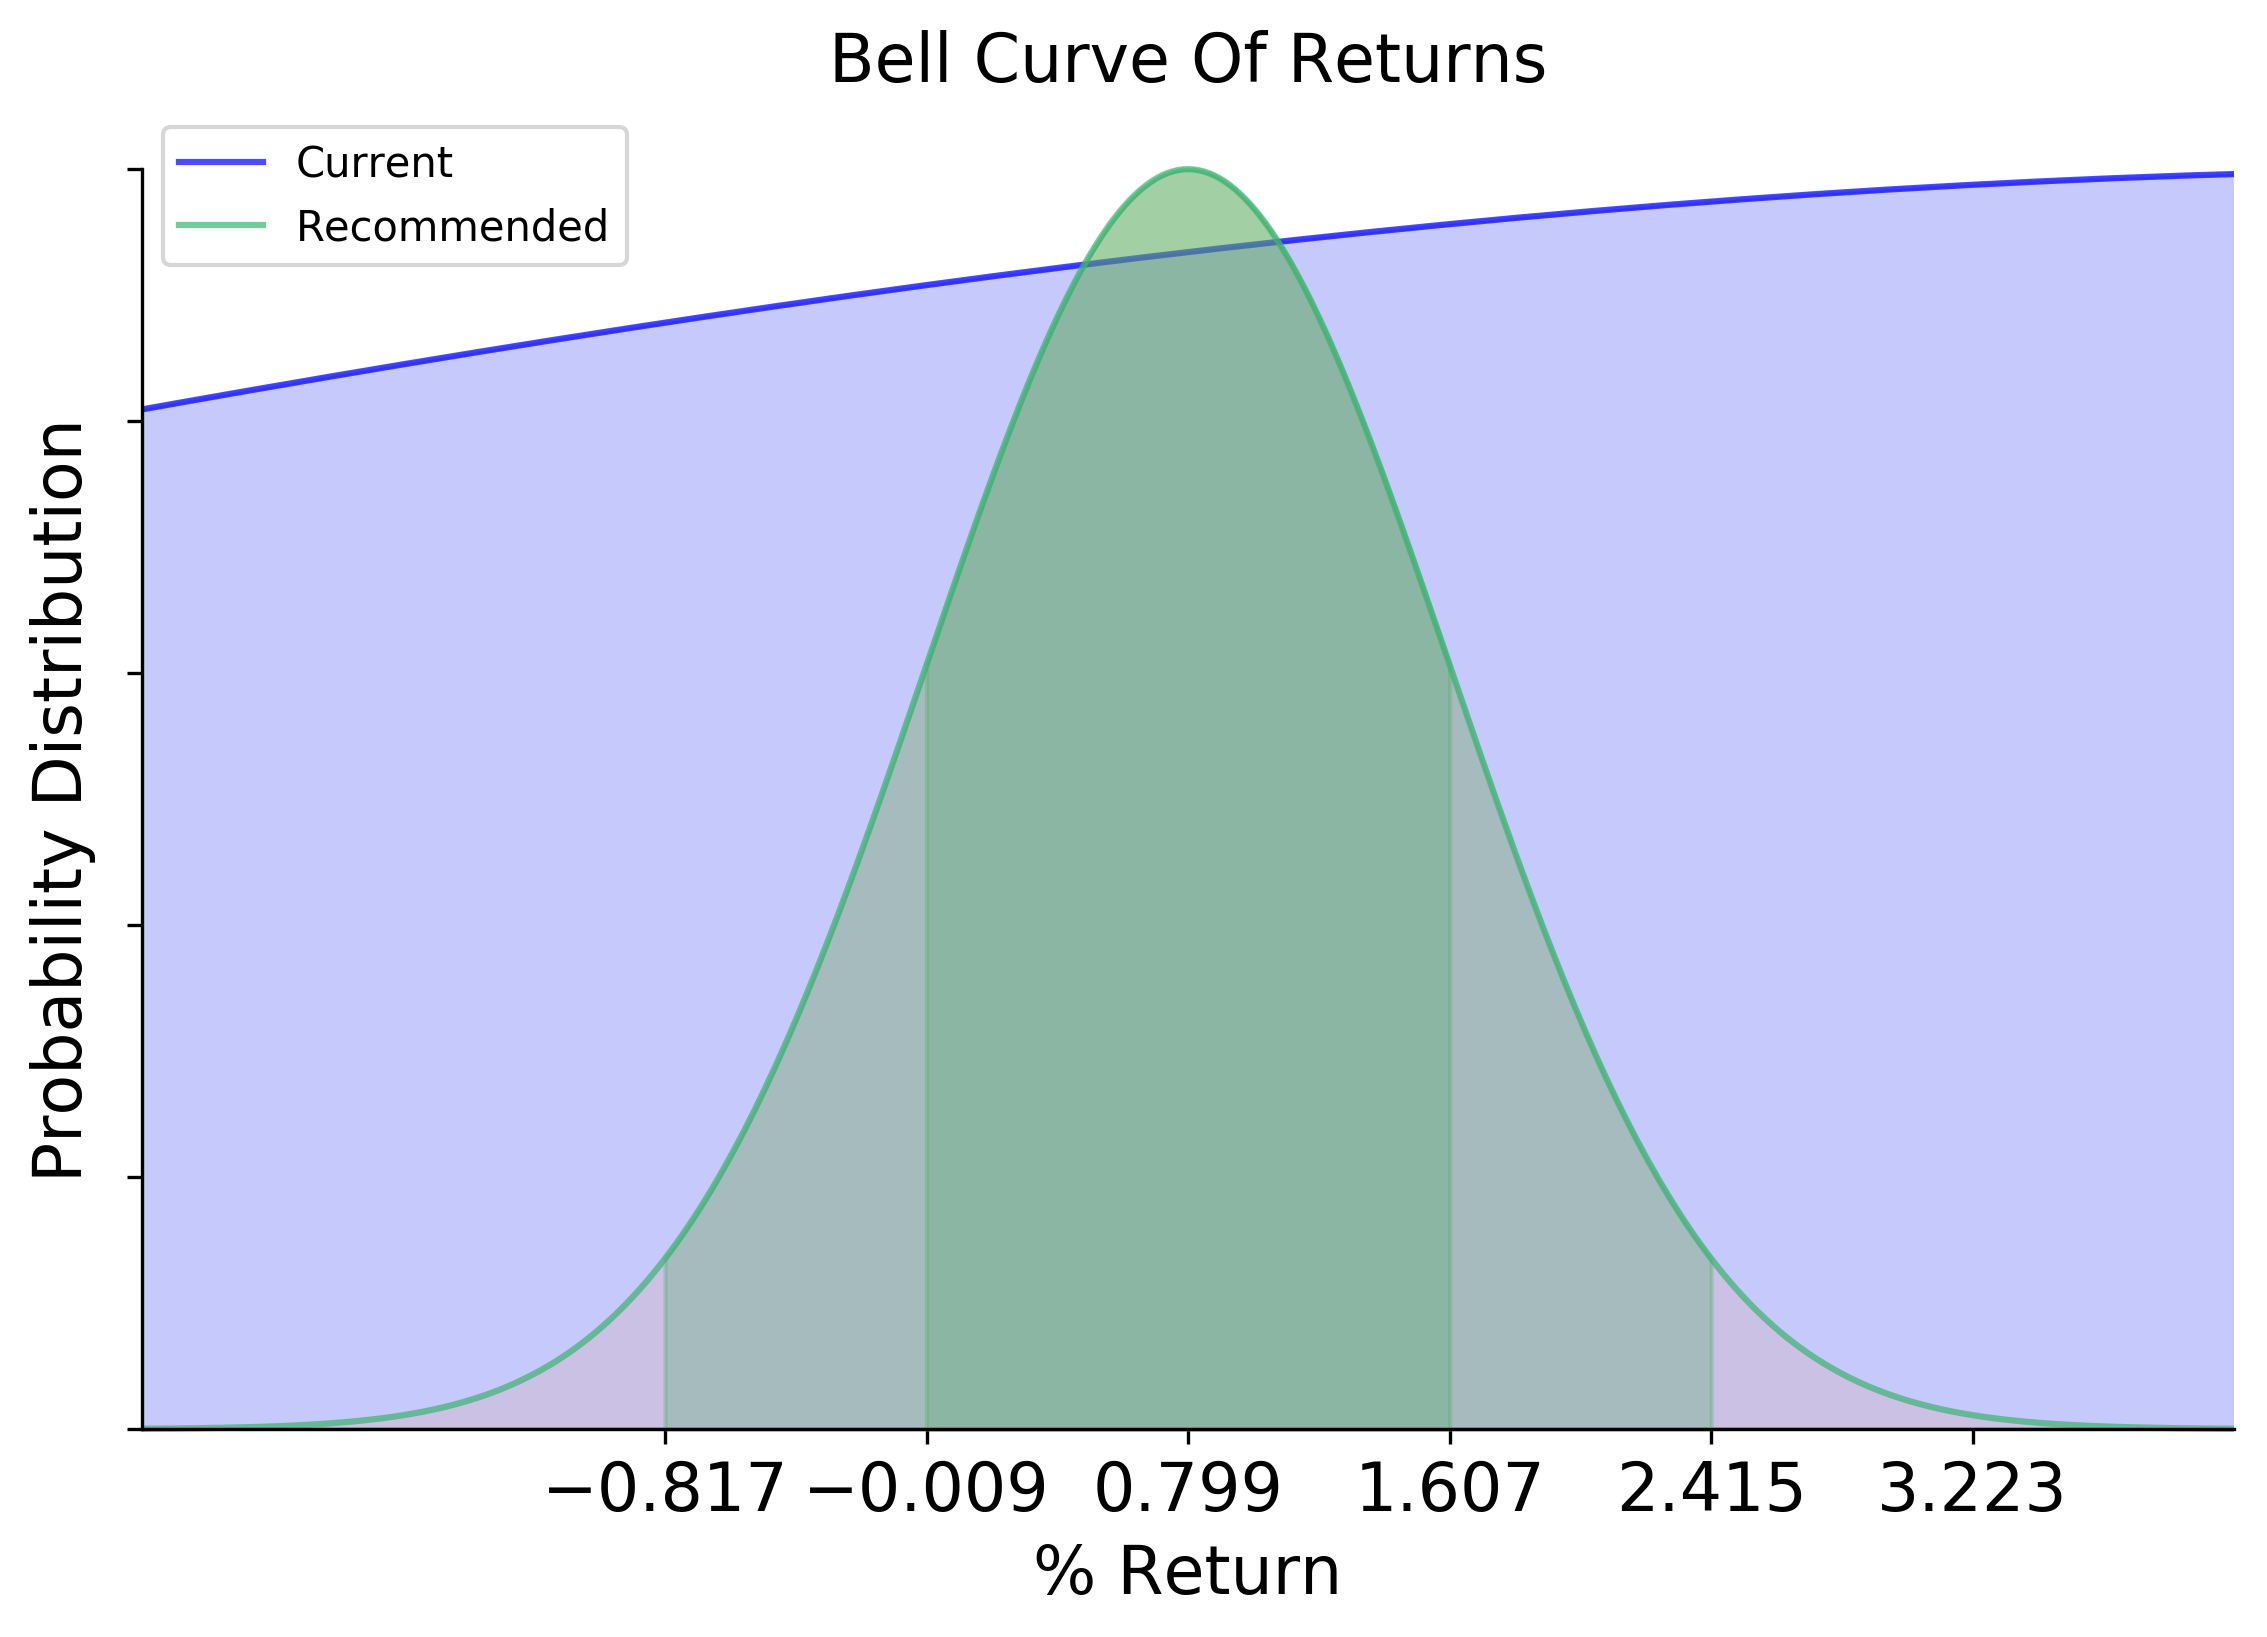
\includegraphics[width=.45\linewidth]{/app/plts/bellcompare.png}
    & \hspace{1cm }&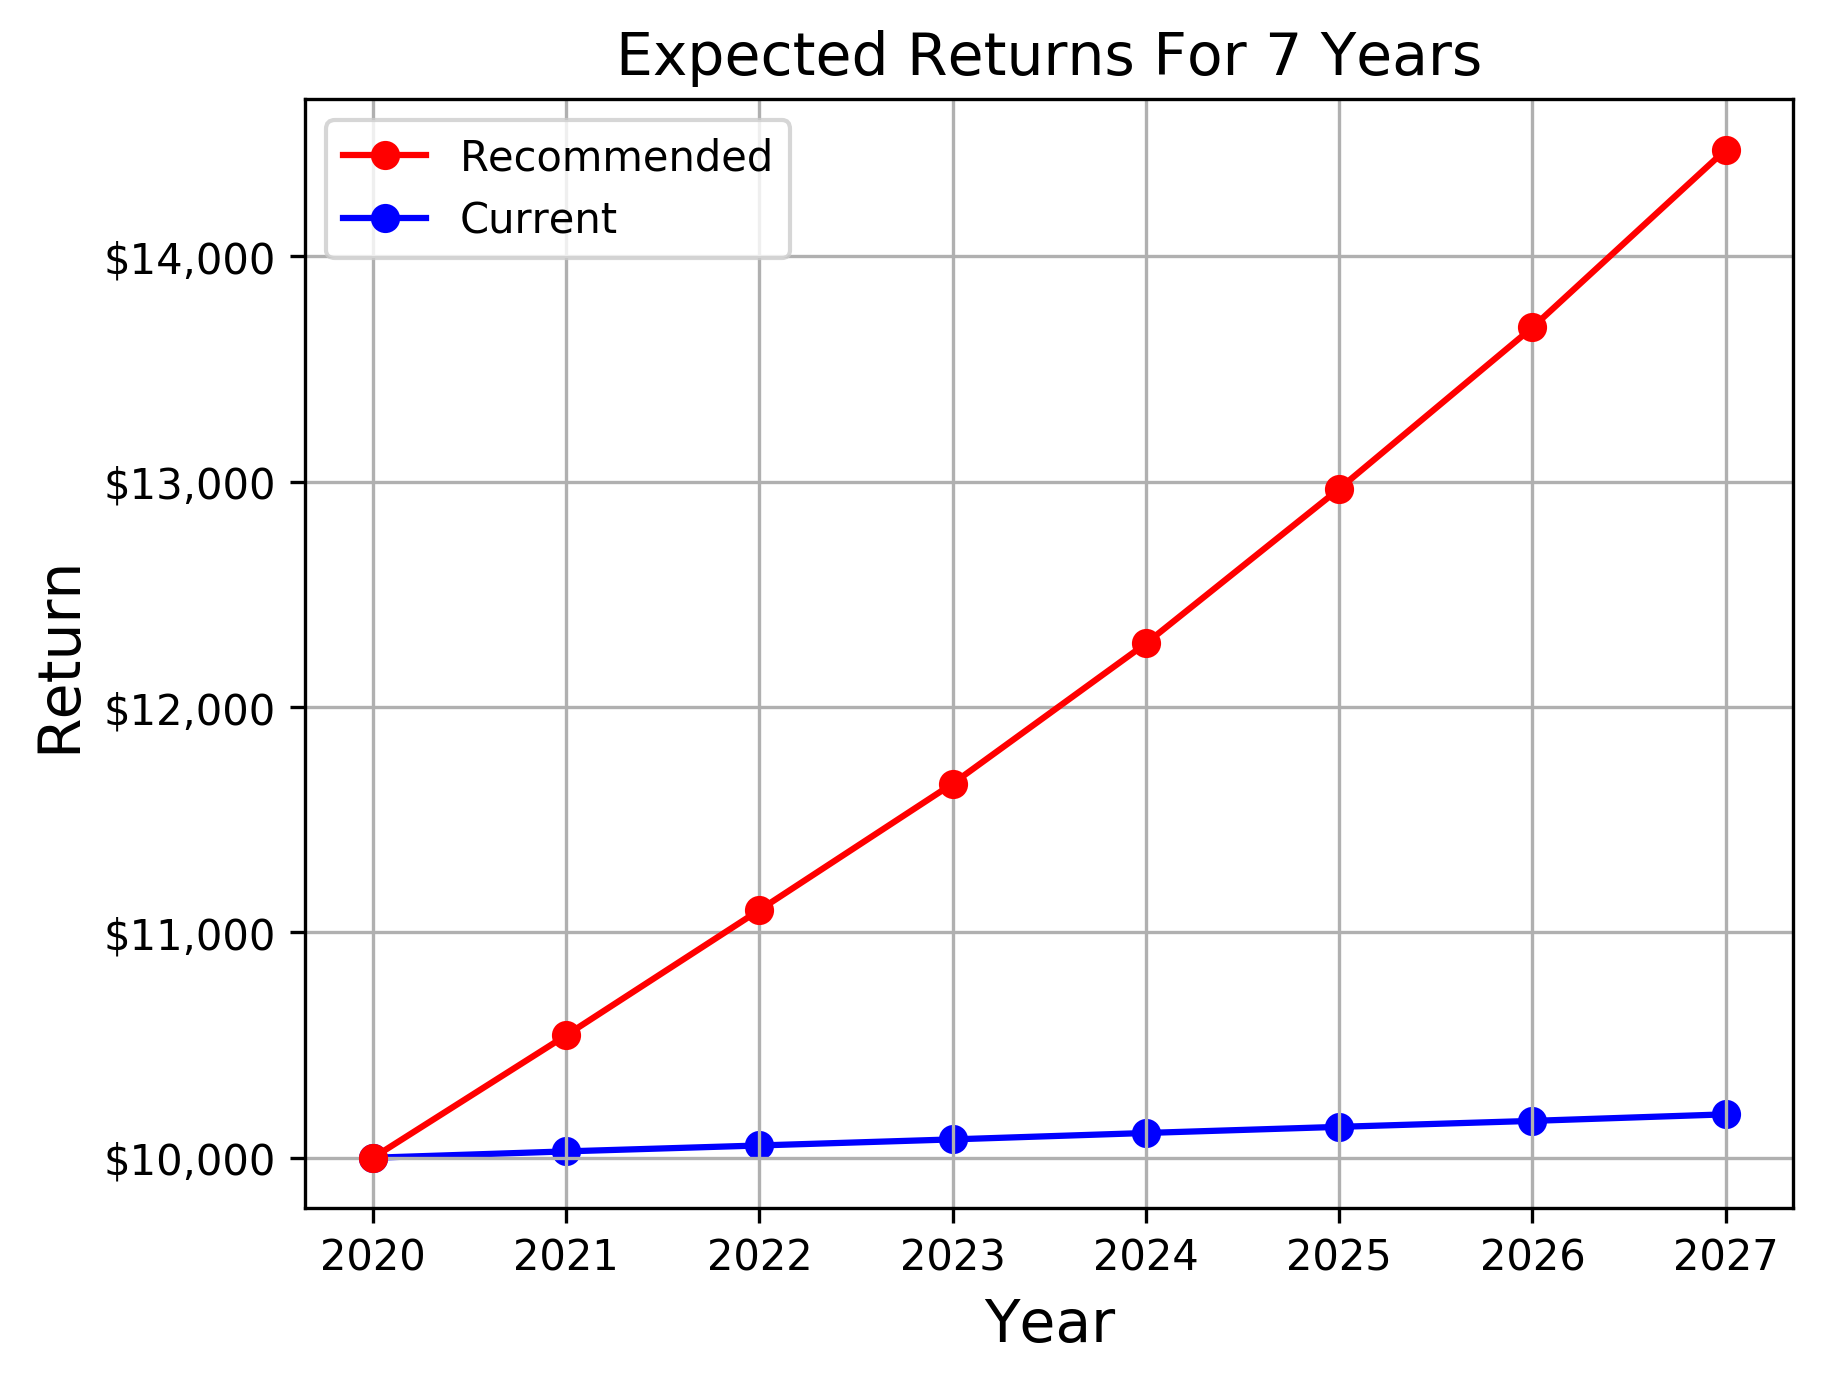
\includegraphics[width=.45\linewidth]{/app/plts/line7.png}
  \end{tabular}
  \end{center}

  \begin{center}
      (b) Current Portfolio 7 Year Projections
      %(a) Returns of Current Portfolio
      %(a) Bell Curves Of Expected Return
  \end{center}

 \vspace{.6cm}

\end{adjustwidth}

\noindent
1 Year Expected Return (\$): {\VAR{info.blueoneret}} \quad \emph{{\VAR{info.blueoneretchange}}} \\
1 Year Risk (Std Deviation \%) : $\pm$ {\VAR{bluerisk}}
\\
\noindent
7 Year Expected Return (\$): {\VAR{info.bluesevenret}} \quad \emph{{\VAR{info.bluesevenretchange}}} \\
7 Year Risk (Std Deviation \%): $\pm$ {\VAR{info.bluesevenrisk}}


\newpage    % PAGE6


\section{Prescribed Portfolio Overview - Statistical Analysis}

\vspace{1.5cm}

%https://tex.stackexchange.com/questions/257337/how-to-have-a-figure-with-multiple-groups-of-image-and-each-image-with-individua

\begin{adjustwidth}{-.3in}{0in}% adjust the L and R margins by 1 inch
\vspace*{-1cm}

\begin{center}
  \begin{tabular}{c}
    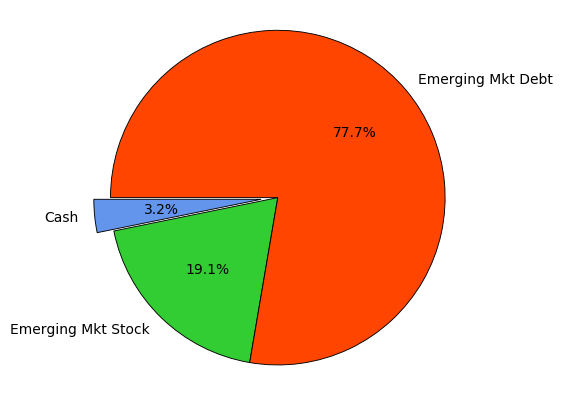
\includegraphics[width=.5\linewidth]{/app/plts/piefuture.png}
  \end{tabular}
  \end{center}

  \begin{center}
        Portfolio Breakdown
      %(b) Projected Returns (Monte Carlo)
  \end{center}

\vspace{.7cm}


\begin{center}
  \begin{tabular}{lcr}
  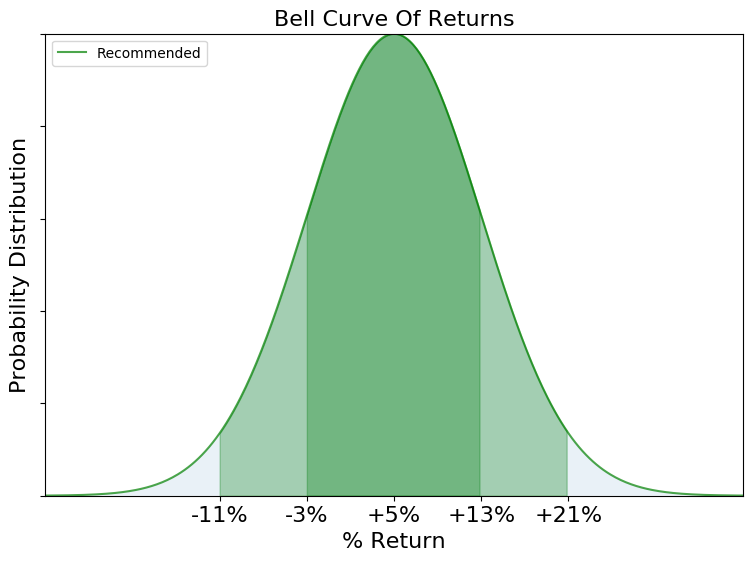
\includegraphics[width=.45\linewidth]{/app/plts/bellfuture.png}
    & \hspace{1cm }&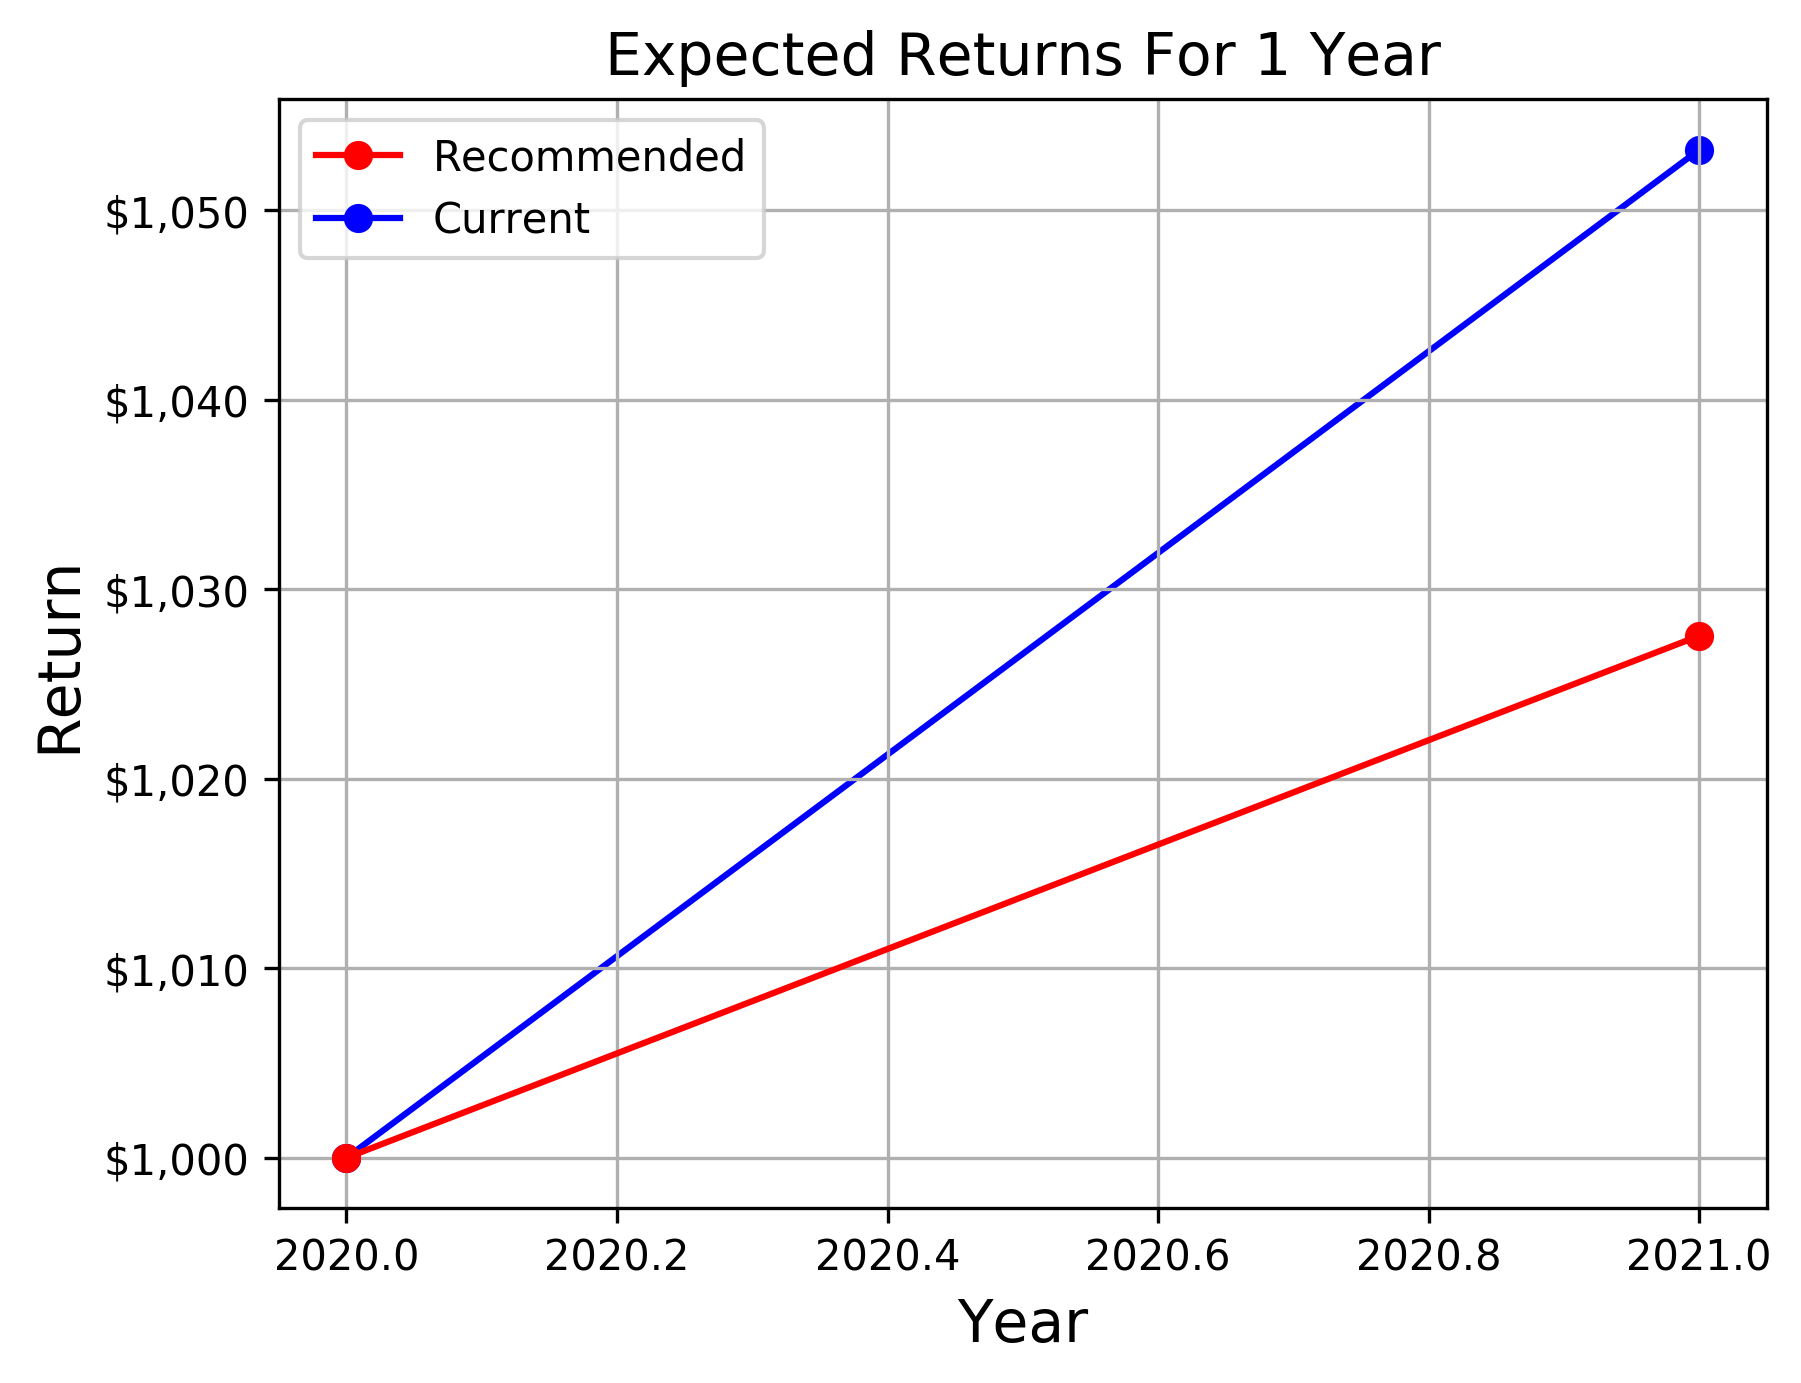
\includegraphics[width=.45\linewidth]{/app/plts/line1.png}
  \end{tabular}
  \end{center}

  \begin{center}
      (a) Prescribed Portfolio 1 Year Projections
      %(a) Returns of Current Portfolio
      %(a) Bell Curves Of Expected Return
  \end{center}

  \vspace{.7cm}


\begin{center}
  \begin{tabular}{lcr}
  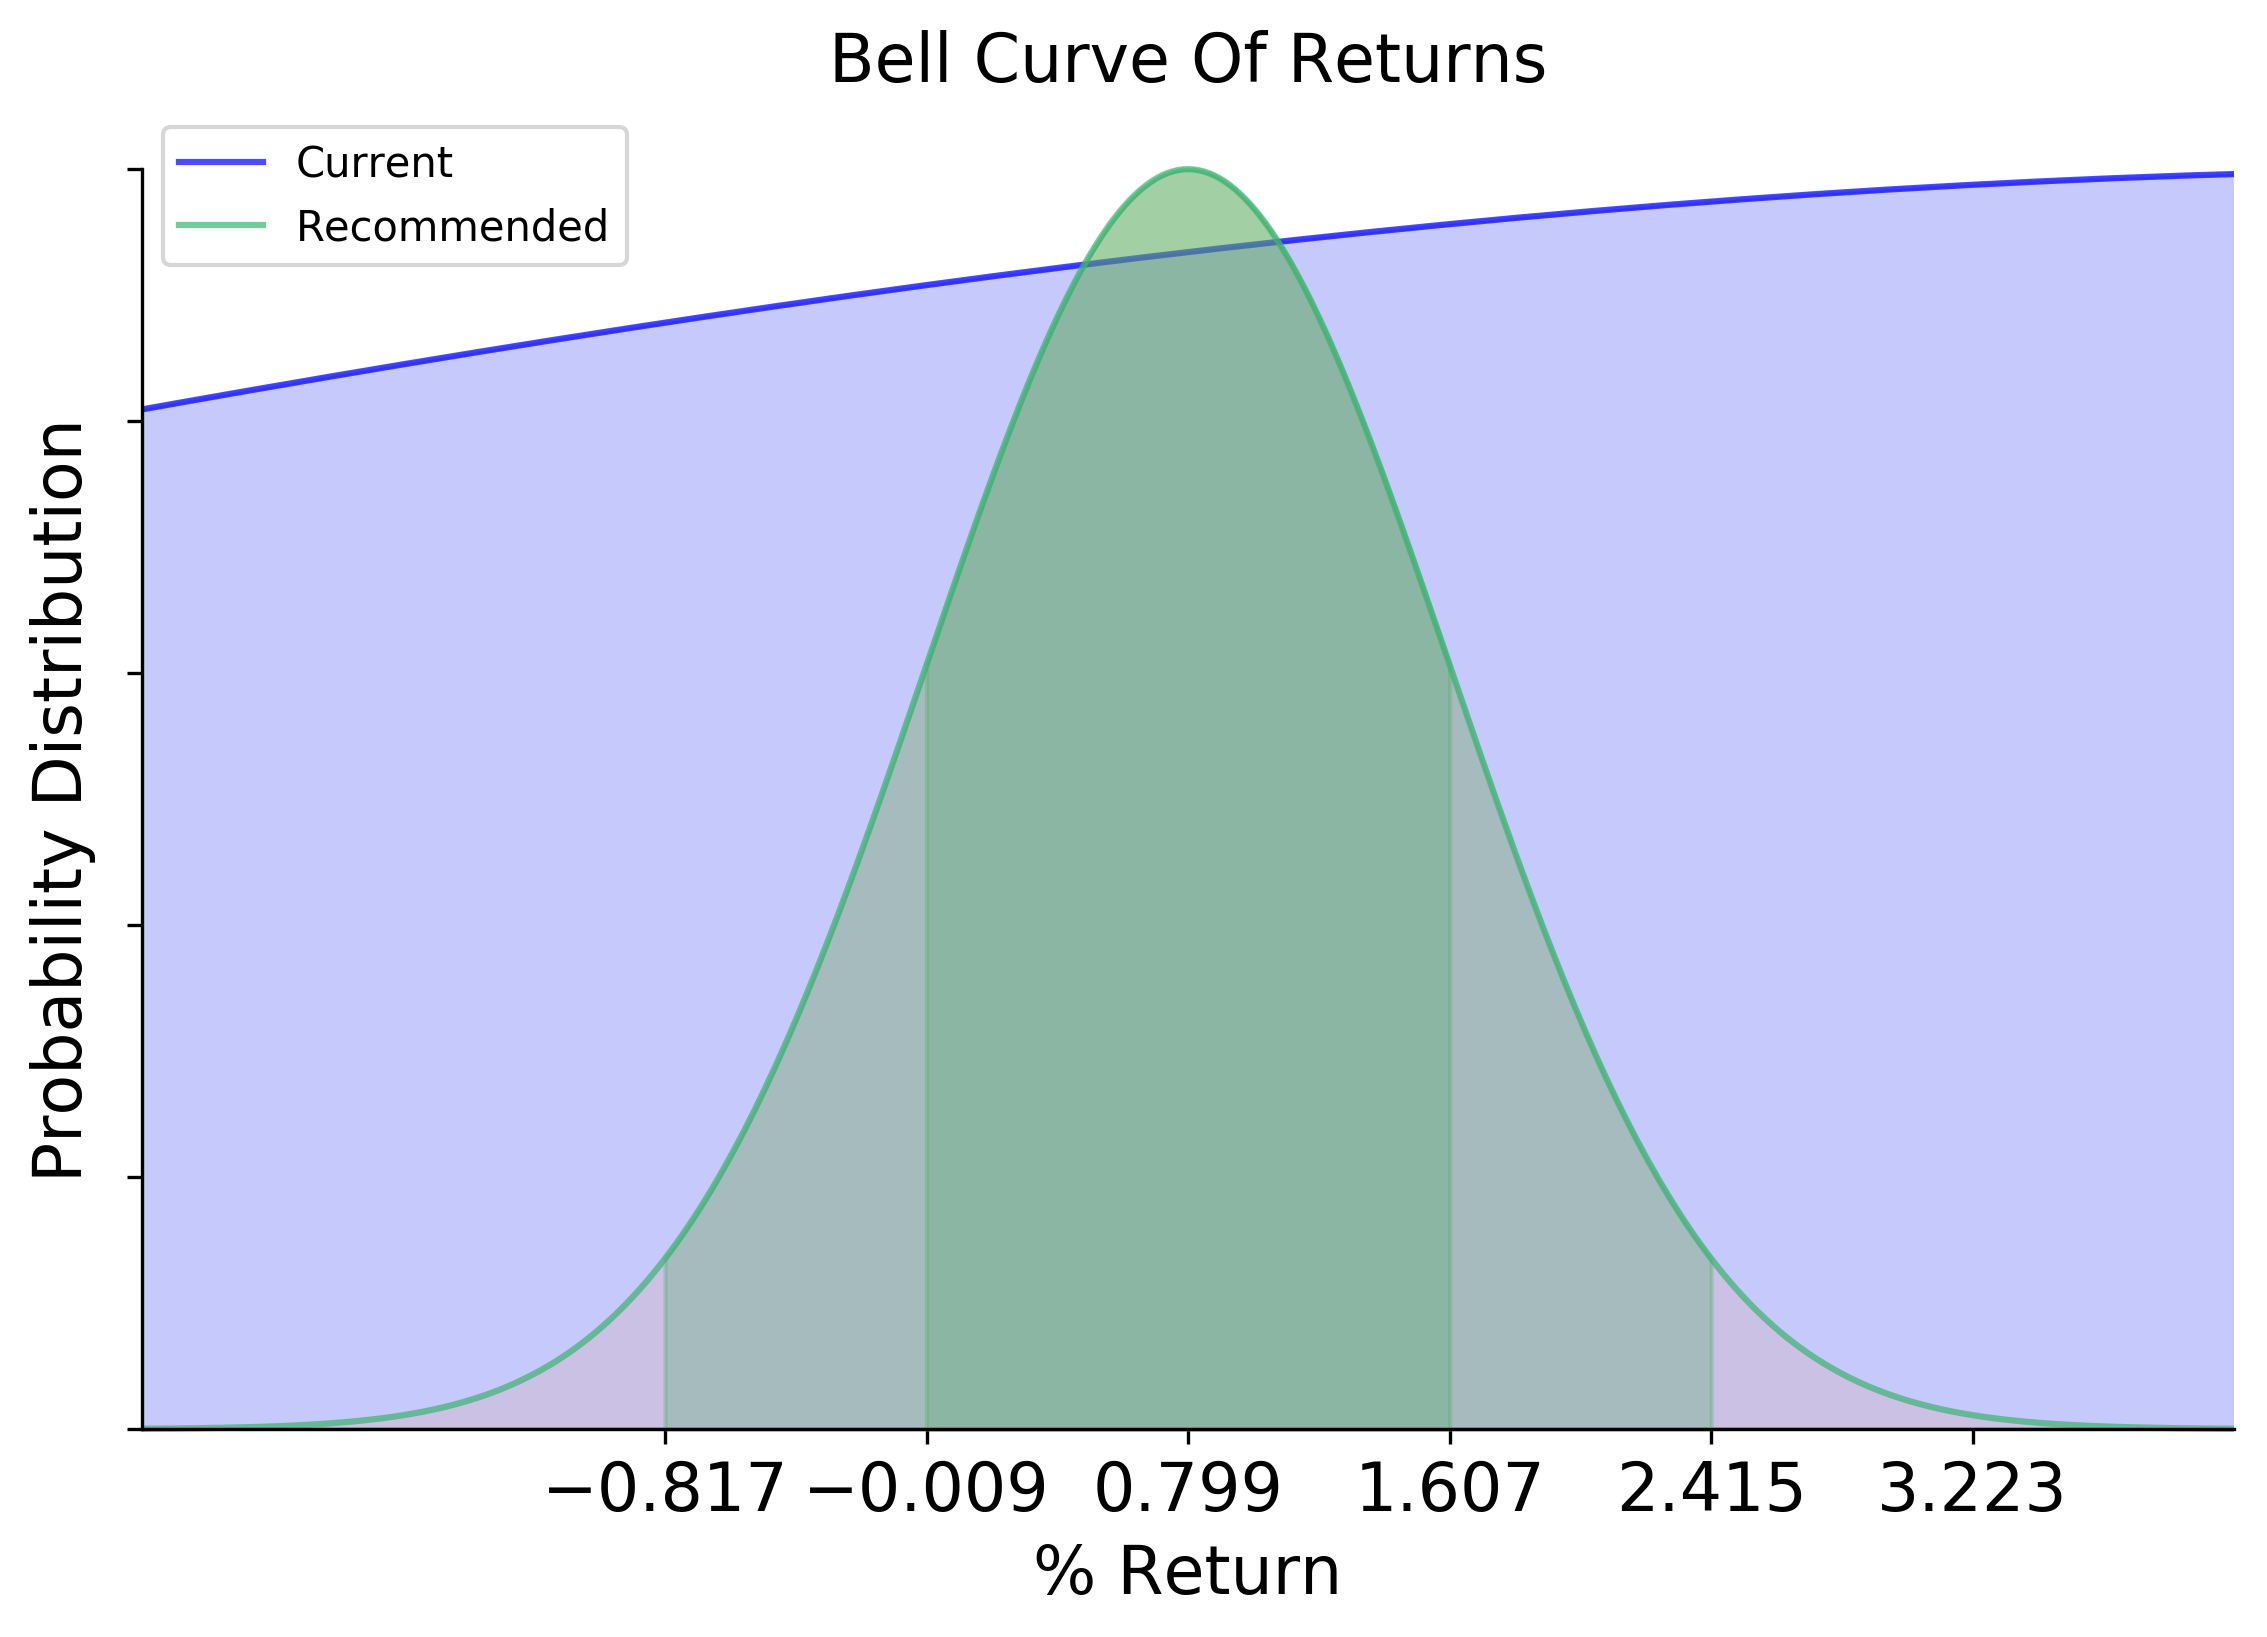
\includegraphics[width=.45\linewidth]{/app/plts/bellcompare.png}
    & \hspace{1cm }&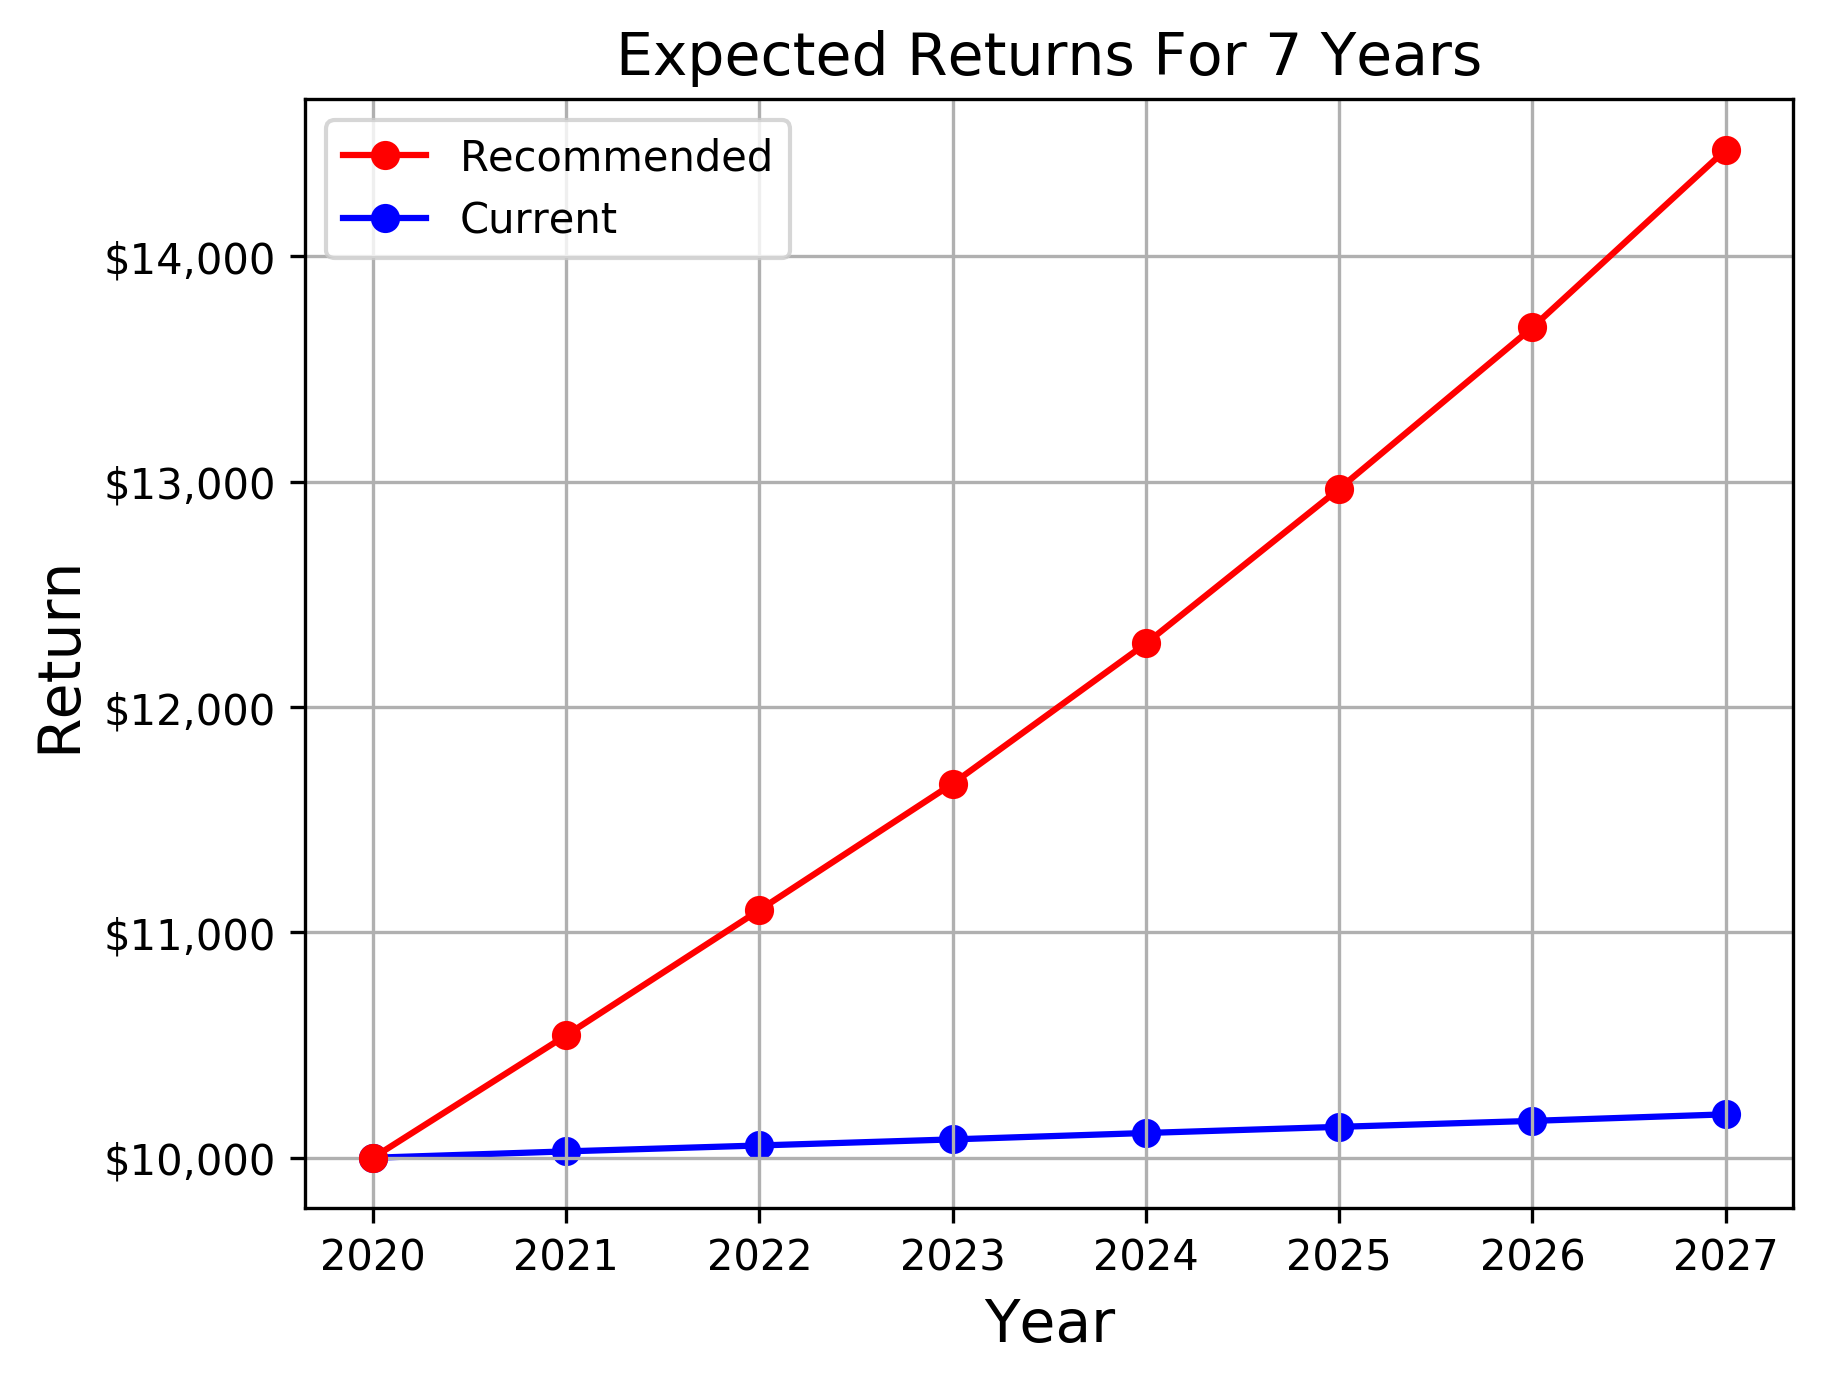
\includegraphics[width=.45\linewidth]{/app/plts/line7.png}
  \end{tabular}
  \end{center}

  \begin{center}
      (b) Prescribed Portfolio 7 Year Projections
      %(a) Returns of Current Portfolio
      %(a) Bell Curves Of Expected Return
  \end{center}

\vspace{.6cm}

\end{adjustwidth}

\noindent
1 Year Expected Return (\$): {\VAR{info.redoneret}} \quad \emph{{\VAR{info.redoneretchange}}}\\
1 Year Risk (Std Deviation \%): $\pm$ {\VAR{redrisk}}
\\
\noindent
7 Year Expected Return (\$): {\VAR{info.redsevenret}} \quad \emph{{\VAR{info.redsevenretchange}}}\\
7 Year Risk (Std Deviation \%): $\pm$ {\VAR{info.redsevenrisk}}



\newpage    % PAGE7



\section{Frontier Curve}

In 1990, Harry Markowitz won a nobel prize for his contributions to portfolio balancing theory. Markowitz discovered that given assets to buy from and funds to buy with, all of the optimal portfolios formed on a curved line called the "Frontier Curve."

\vspace{2cm}

\hspace*{-2.5cm}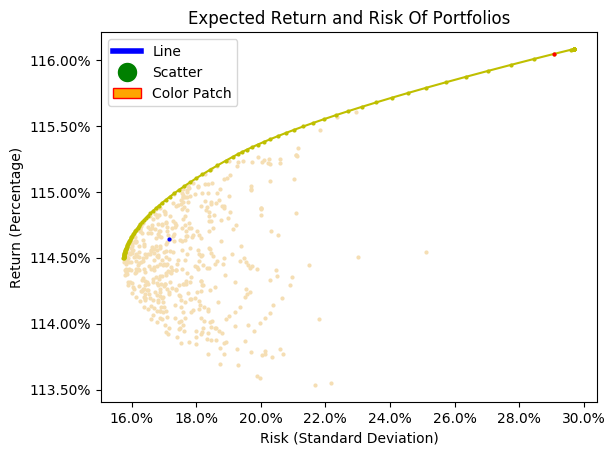
\includegraphics[width=1.2\linewidth]{/app/plts/frontier.png}\par

\vspace{1cm}

Risk (Std. Deviation): $\pm$ {\VAR{redrisk}}

Expected Return (\%): {\VAR{redret}}

Adjustment of Risk (\%): {\VAR{riskchange}}

Change in Return (\%): {\VAR{retchange}}


\newpage    % PAGE8

\begin{landscape}

\section{Correlation Matrix}

\vspace{1cm}

\begin{center}


\scriptsize
        \VAR{C}
\vspace{0.3cm}

    Above is the Semantic Correlation Matrix of the selected Asset Classes. It shows how each asset class is correlated to one another

\end{center}


\vspace{1cm}

\newpage  %PAGE9

\section{Risk \& Return Rankings}

\vspace{2cm}

\begin{center}

    \VAR{r}
\vspace{0.3cm}

    Above is the ranking of the selected asset classes by risk

\end{center}







\vspace{1cm}


\begin{center}

    \VAR{p}
    \vspace{0.3cm}

    Above is the ranking of the selected asset classes by return

\end{center}

\end{landscape}
\newpage
\begin{center}
{\scshape\Large\bfseries \, \par}
	\vspace{10cm}
\emph{Intentionally Left Blank}

\end{center}
\end{document}




